%% ===================================================================
%% Cover letter body
%% ===================================================================
%% \lipsum is provided by the lipsum package for generating placeholder text.
%% [1-3] specifies the range of paragraphs to be included.

%% ---- Typography settings ----
\tolerance=1000
\emergencystretch=3em
\hyphenpenalty=500
\exhyphenpenalty=10000

%% ---- Main content ----
\begin{document}
\begin{frame}[t]
\fontsize{32}{36}\selectfont

%% ---- The first column ----
\begin{columns}[t]
\separatorcolumn

\begin{column}{\colwidth}
  %% ---- Abstract ----
  \begin{block}{Abstract}
    This poster demonstrates how to use the \textbf{WestlakeU-LaTeX Poster Template} to create 
    professional academic posters. The template is built on the \texttt{beamerposter} package 
    and provides a clean, structured layout with customizable colors, fonts, and blocks. 
    This guide walks through the key features including section organization, typography, 
    mathematics, tables, algorithms, figures, and references.
  \end{block}

 \begin{alertblock}{Key Features}

   This poster template offers the following capabilities:

   \begin{itemize}
     \item \textbf{Multiple Block Types:} Use \texttt{block} for standard content, 
           \texttt{alertblock} for highlights, and \texttt{exampleblock} for examples.

     \item \textbf{Flexible Layout:} Two-column design with adjustable column width 
           and separator spacing via \texttt{\textbackslash colwidth} and \texttt{\textbackslash sepwidth}.

     \item \textbf{Custom Branding:} Add logos via \texttt{\textbackslash logoleft} and 
           \texttt{\textbackslash logoright}, and set footer content with \texttt{\textbackslash footercontent}.
   \end{itemize}

 \end{alertblock}

  %% ---- Methods ----
  \begin{block}{Methods}
    %% ---- Typography ----
    \heading{Getting Started}
    Key commands you will use frequently in \texttt{content.tex} include:

    \begin{table}
      \centering
      \begin{tabular}{lll}
        \texttt{\textbackslash heading} & \texttt{\textbackslash subsection} & \texttt{\textbackslash subsubsection}\\
        \texttt{\textbackslash centering} & \texttt{\textbackslash includegraphics} & \texttt{\textbackslash caption}\\
        \texttt{\textbackslash cite} & \texttt{\textbackslash ref} & \texttt{\textbackslash label}\\
      \end{tabular}
      \caption{Common \LaTeX\ commands}
    \end{table}

    %% ---- Referencing ----
    \heading{Referencing and Hyperlinks}
    Cite references using \texttt{\textbackslash cite} with keys from your \texttt{.bib} file. The template supports articles, books, websites, and conference papers. \\
    Referencing: Use \texttt{\textbackslash ref} to link to figures, tables, and equations. \\
    Hyperlinks: Use \texttt{\textbackslash url} or \texttt{\textbackslash href} 
    for external links, e.g., \url{https://www.westlake.edu.cn}.

    %% ---- Mathematics ----
    \heading{Working with Mathematics}
        \LaTeX\ excels at typesetting mathematical formulas. Use \textit{inline} mode 
    (\texttt{\$...\$}) for inline expressions like $E=mc^2$, and \textit{display} 
    mode for numbered or unnumbered equations:

    \begin{equation}
        p^{*}(y_{w}\succ y_{l} \mid x) = \frac{\exp(r^{*}(x,y_{w}))}{\exp(r^{*}(x,y_{w}))+\exp(r^{*}(x,y_{l}))}. \label{eq:poster1}
    \end{equation}

    For multi-line alignment, use the \texttt{align*} environment:

    \begin{align*}
        \mathbb{D}_{\text{KL}}(P || Q) = \sum_{x \in \mathcal{X}} P(x)\log \left( \frac{P(x)}{Q(x)} \right)
    \end{align*}

    %% ---- Algorithms ----
    \heading{Algorithm}

    \begin{pseudoalgorithm}{Generative Adversarial Imitation Learning (GAIL)}
    \begin{algorithmic}[1]
        \State Input: Expert trajectories $\tau_E \sim \pi_E$, initial policy and discriminator parameters $\theta_0, w_0$
        \For{$i=0,1,2, \ldots$}
            \State Sample trajectories $\tau_i \sim \pi_{\theta_i}$
            \State Update the discriminator parameters from $w_i$ to $w_{i+1}$ with the gradient
            $$
                \hat{\mathbb{E}}_{\tau_i}\left[\nabla_w \log \left(D_w(s, a)\right)\right]+\hat{\mathbb{E}}_{\tau_E}\left[\nabla_w \log \left(1-D_w(s, a)\right)\right]
            $$
            \State Take a policy step from $\theta_i$ to $\theta_{i+1}$, using the TRPO rule with cost function $\log \left(D_{w_{i+1}}(s, a)\right)$. Specifically, take a KL-constrained natural gradient step with
            \begin{align*}
                & \hat{\mathbb{E}}_{\tau_i}\left[\nabla_\theta \log \pi_\theta(a \mid s) Q(s, a)\right]-\lambda \nabla_\theta H\left(\pi_\theta\right), \\
                & \text { where } Q(\bar{s}, \bar{a})=\hat{\mathbb{E}}_{\tau_i}\left[\log \left(D_{w_{i+1}}(s, a)\right) \mid s_0=\bar{s}, a_0=\bar{a}\right]
            \end{align*}
        \EndFor
        \end{algorithmic}
    \end{pseudoalgorithm}
  \end{block}

\end{column}

\separatorcolumn

%% ---- The second column ----
\begin{column}{\colwidth}
  %% ---- Results ----
  \begin{block}{Results}
    Use the \texttt{table} environment with \texttt{booktabs} to create three-line tables. Below is an example:

    \begin{table}
      \centering
      \caption{Experimental results comparison across methods.}
      \label{tab:results1}
      \begin{tabular}{lcccc}
        \toprule
        \textbf{Method} & \textbf{Accuracy (\%)} & \textbf{Precision (\%)} & \textbf{Recall (\%)} & \textbf{F1-score (\%)} \\
        \midrule
        Baseline       & 82.3 & 80.1 & 79.5 & 79.8 \\
        Ours    & \textbf{92.1} & \textbf{91.5} & \textbf{91.0} & \textbf{91.2} \\
        Ablation A     & 88.4 & 87.0 & 86.8 & 86.9 \\
        Ablation B     & 90.2 & 89.8 & 89.3 & 89.5 \\
        \bottomrule
      \end{tabular}
    \end{table}

    Use the \texttt{figure} environment with \texttt{\textbackslash includegraphics} 
    to insert images. Below is an example:

    \begin{figure}
      \centering
      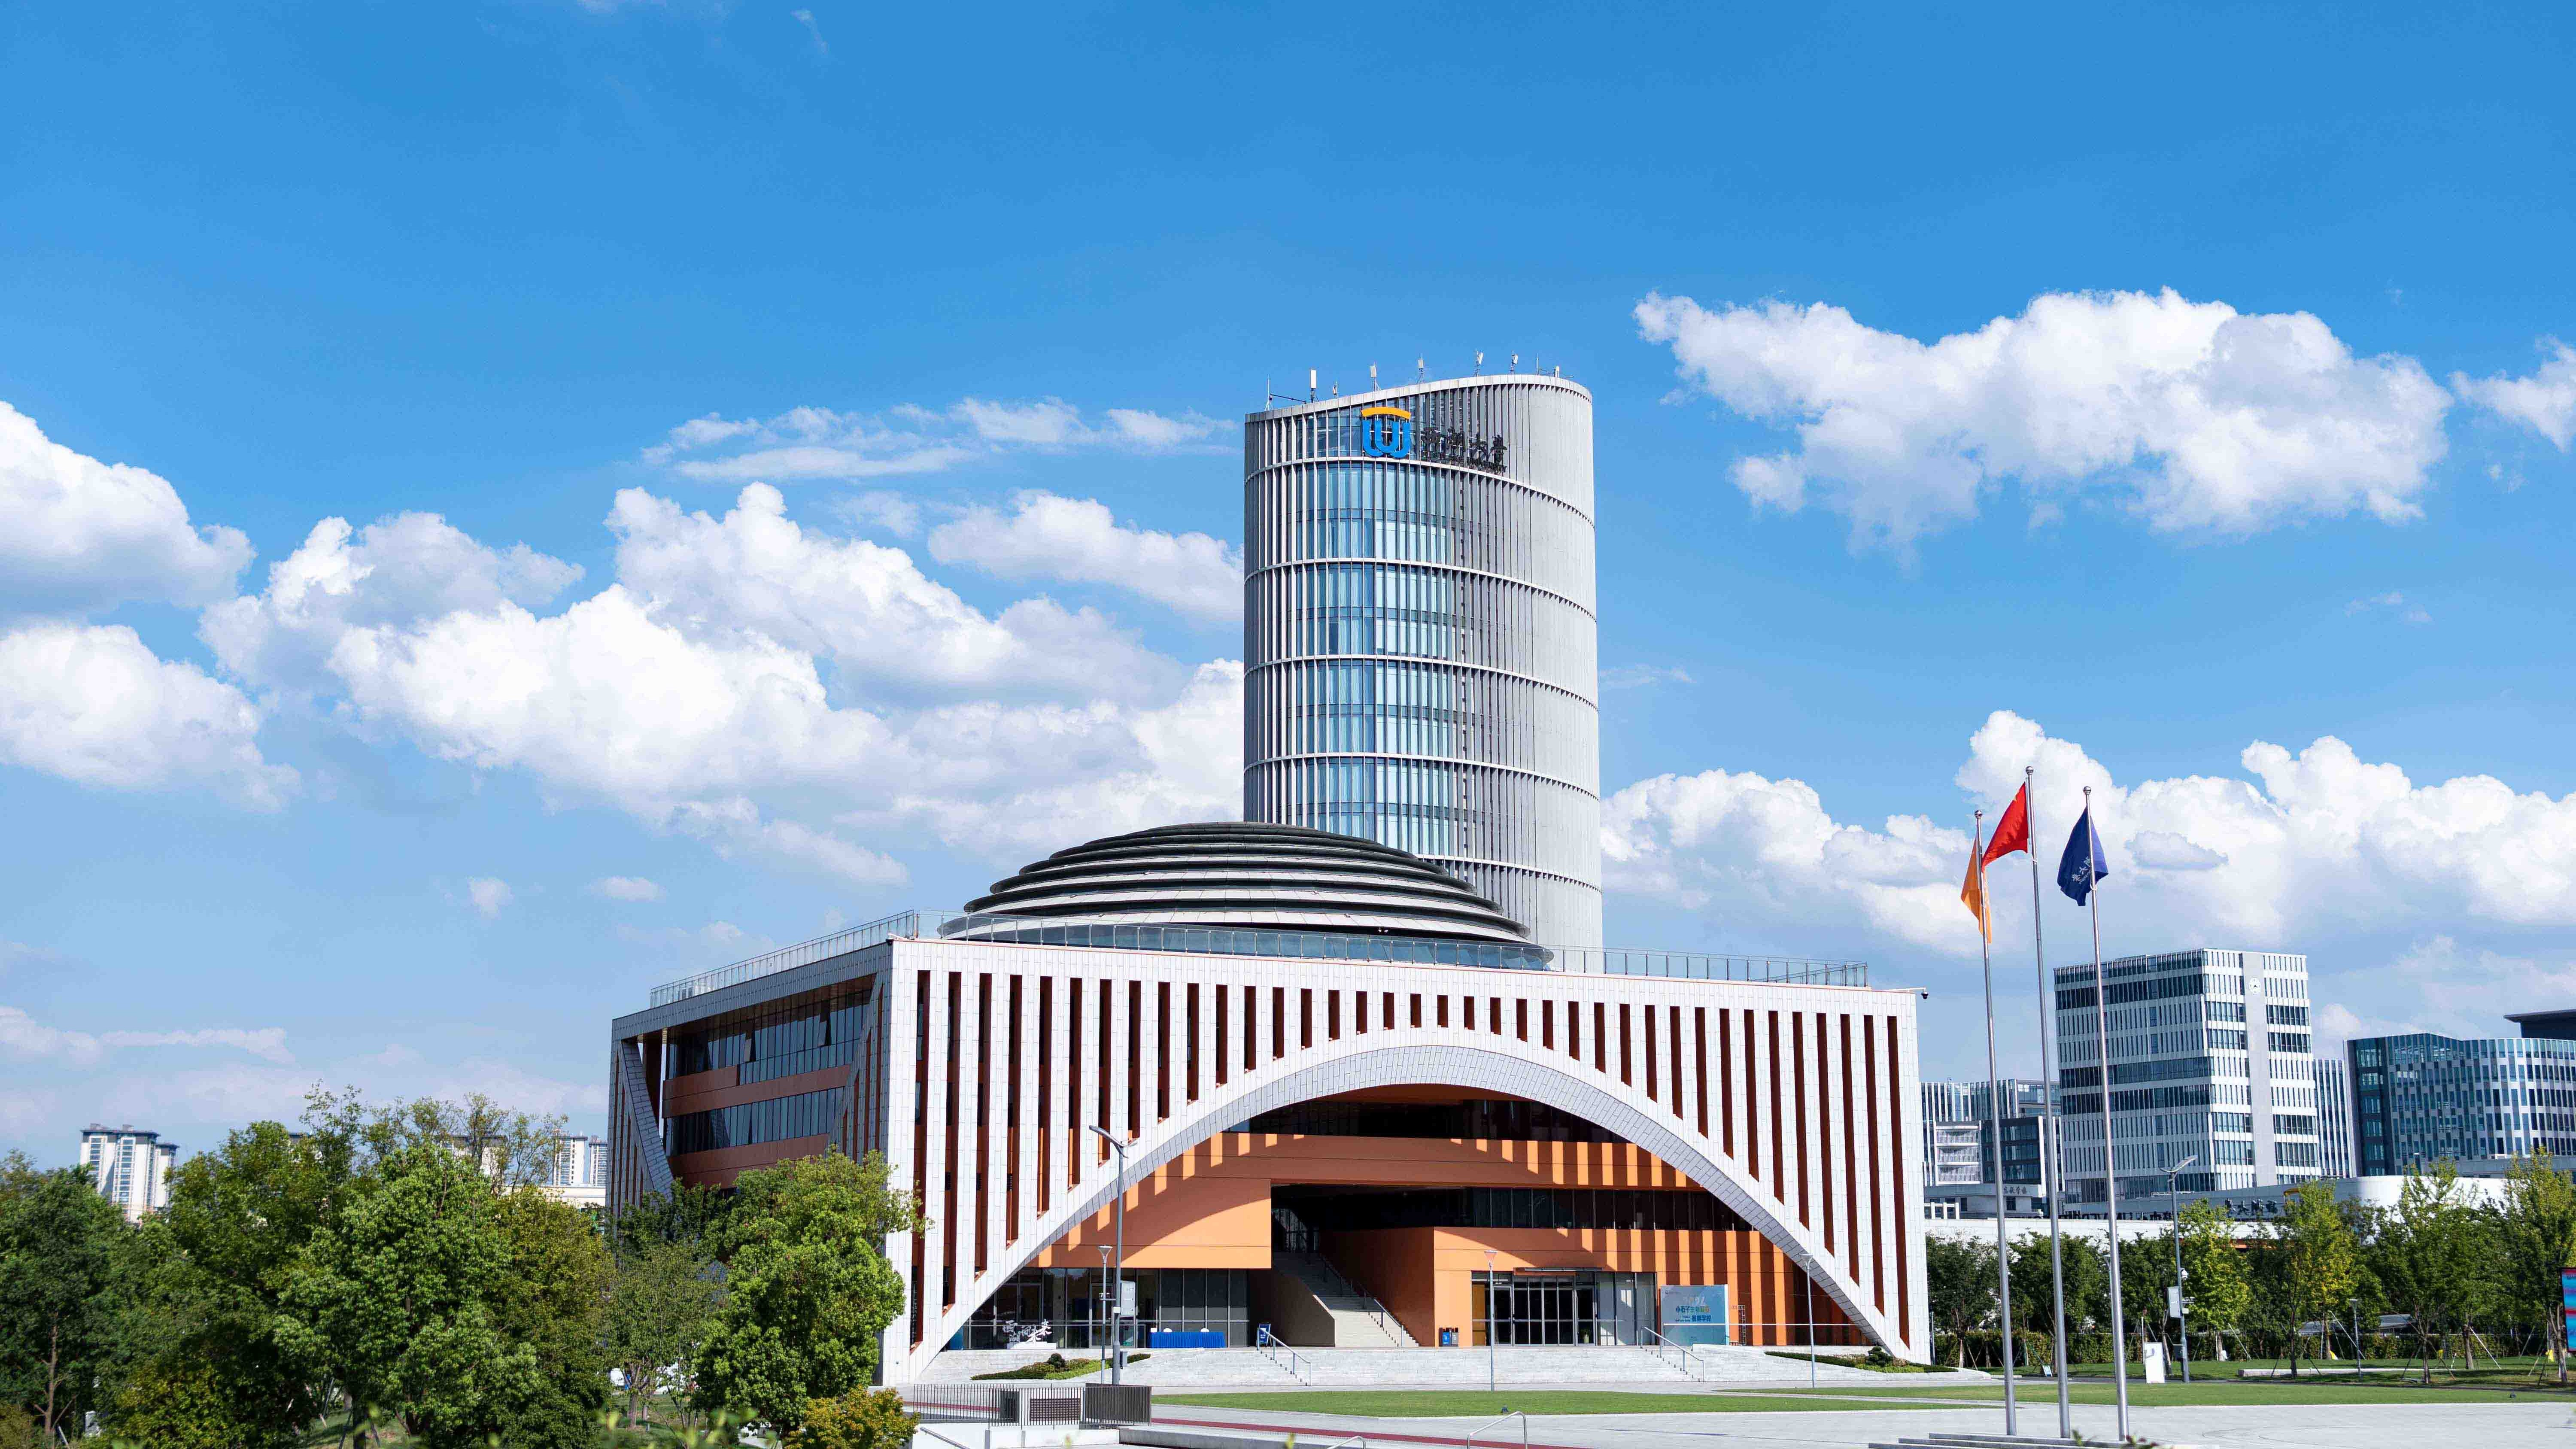
\includegraphics[width=0.9\colwidth]{../../assets/photo.jpg}
      \caption{Photo taken at Westlake University.}
      \label{fig:fig1}
    \end{figure}

    \begin{figure}
      \centering
      \begin{tikzpicture}[scale=3.2]
        % Grid
        \draw[very thin, gray!30, dotted] (-0.5,-1.5) grid (7.5,1.5);
        % Axes
        \draw[->, >=stealth, thick, -{Stealth[scale=1.8]}] (-0.5,0) -- (7.8,0) node[below right, font=\large] {$x$};
        \draw[->, >=stealth, thick, -{Stealth[scale=1.8]}] (0,-1.6) -- (0,1.7) node[above left, font=\large] {$y$};
        % Ticks
        \foreach \x in {1,2,3,4,5,6,7}
          \draw[thick] (\x,2pt) -- (\x,-2pt) node[below, font=\small] {$\x$};
        \foreach \y in {-1,1}
          \draw[thick] (2pt,\y) -- (-2pt,\y) node[left, font=\small] {$\y$};
        \node at (-2pt,0) [below left, font=\small] {$0$};
        % Sine curve
        \draw[domain=0:7, smooth, variable=\x, westlakeblue, thick] plot ({\x}, {sin(\x r)});
        % Axis label
        \node[above, font=\large\bfseries, westlakeblue] at (3.5, 1.55) {$y = \sin(x)$};
        % Filled dot at origin
        \filldraw[westlakeblue] (0,0) circle (2pt);
      \end{tikzpicture}
      \caption{Sine curve drawn with TikZ, showing key features including axes, grid, and labeled ticks.}
      \label{fig:tikz1}
    \end{figure}

  \end{block}

  %% ---- Conclusions ----
  \begin{exampleblock}{Conclusions}
    \begin{itemize}
      \item This \textbf{WestlakeU-LaTeX Poster Template} provides a clean, professional layout for academic posters using the \texttt{beamerposter} package.
      \item Customize colors via \texttt{\textbackslash definecolor} and block styles through \texttt{\textbackslash setbeamercolor} in \texttt{westlakeu-poster.sty}.
      \item The two-column layout adapts automatically --- adjust \texttt{\textbackslash colwidth} and \texttt{\textbackslash sepwidth} for your content needs.
      \item Add your own logo with \texttt{\textbackslash logoleft} and \texttt{\textbackslash logoright}; set footer information via \texttt{\textbackslash footercontent}.
      \item All content goes into \texttt{content.tex} --- simply replace the placeholder text, figures, and references with your own.
    \end{itemize}
  \end{exampleblock}

  %% ---- Acknowledgements ----
  \begin{block}{Acknowledgements}
    This poster template is built on \texttt{beamerposter} and the \texttt{WestlakeU-LaTeX} project. Special thanks to all contributors who helped improve the design and usability. For questions or suggestions, please visit the project repository or contact the maintainers.
  \end{block}

\end{column}

\separatorcolumn
\end{columns}

\end{frame}